% 设置 biblatex 额外选项
% \PassOptionsToPackage{gbpub=false, gbtype=false}{biblatex}

% 载入 SJTUThesis 模版
% \documentclass[degree=doctor, zihao=-4, language=english, review]{sjtuthesis}
% \documentclass[degree=master, zihao=-4]{sjtuthesis}
\documentclass[degree=bachelor, openany, oneside]{sjtuthesis}
% \documentclass[degree=course, language=english, openright, twoside]{sjtuthesis}
% 选项
%   degree=[doctor|master|bachelor|course],     % 必选,学位类型
%   language=[chinese|english],                 % 可选(默认:chinese),论文的主要语言
%   bibstyle=[gb7714-2015|gb7714-2015ay|ieee],  % 可选(默认:gb7714-2015),参考文献样式
%   review,                                     % 可选(默认:关闭),盲审模式

% 所有其它可能用到的包都统一放到这里了,可以根据自己的实际添加或者删除。
\usepackage{sjtuthesis}

% 定义图片文件目录与扩展名
\graphicspath{{figure/}}
\DeclareGraphicsExtensions{.pdf,.eps,.png,.jpg,.jpeg}

% 导入参考文献数据库
\addbibresource{bib/thesis.bib}

% 信息录入,必须在导言区进行!
% !TEX root = ../thesis.tex

%TC:ignore

\title{关于深度学习视频流推理任务的通用编程框架的研究}
\author{梁若凡}
\studentid{516030910383}
\supervisor{冷静文 特别副研究员}
% \assisupervisor{某某教授}
\degree{工学学士}
\major{计算机科学与技术}
\department{电子信息与电气工程学院}
\coursename{某某课程}
\date{2020年05月25日}
% \fund{国家 973 项目 (No. 2025CB000000) \\ 国家自然科学基金 (No. 81120250000)}
\keywords{深度学习, 视频流处理,编程框架, 并行优化}

\entitle{A Sample Document for \LaTeX-based SJTU Thesis Template}
\enauthor{Mo Mo}
\ensupervisor{Prof. Mou Mou}
% \enassisupervisor{Prof. Uom Uom}
\endegree{Master of Engineering}
\enmajor{A Very Important Major}
\endepartment{Depart of XXX}
\endate{Dec. 17th, 2014}
% \enfund{National Basic Research Program of China (Grant No. 2025CB000000) \\
%   National Natural Science Foundation of China (Grant No. 81120250000)}
\enkeywords{SJTU, master thesis, XeTeX/LaTeX template}

%TC:endignore


% 自定义项目标签名称
% \sjtuSetLabel{
%   listfigure = {图\quad 录},
%   listtable  = {表\quad 录}
% }

\begin{document}

% 无编号内容:中英文论文封面、授权页
\maketitle
% \makeDeclareOriginality[pdf/originality.pdf]
\makeDeclareAuthorization

% 使用罗马数字对前言编号
\frontmatter

% 摘要
% !TEX root = ../thesis.tex

\begin{abstract}
深度学习相关软、硬技术在近年来飞速发展使得对视频流内容进行连续的智能分析与推理成为了可能。准确、高效的智能视频分析、理解对未来生产生活的方方面面都有着及其重要的应用价值。然而深度学习相关的视频流处理往往有着较为复杂的计算流程,十分依赖不同模块/代码库的协同计算,有一定的开发门槛与上手难度。此外,深度学习方法目前相比仍然需要数倍于传统视觉算法的计算开销,这种高计算开销也导致了深度学习视频处理任务难以在一般硬件上取得较高的帧率。
% 深度学习技术近年来在计算机视觉领域取得了显著的成就,其相关的计算机视觉算法已经逐步应用到了各类现实应用或生产过程之中。视觉算法性能以及硬件算力的不断提升使得对视频流内容进行连续的智能分析与推理成为了可能。
\end{abstract}

\begin{enabstract}
  Shanghai Jiao Tong University (SJTU) is a key university in China. SJTU was
  founded in 1896. It is one of the oldest universities in China. The University
  has nurtured large numbers of outstanding figures include JIANG Zemin, DING
  Guangen, QIAN Xuesen, Wu Wenjun, WANG An, etc.

  SJTU has beautiful campuses, Bao Zhaolong Library, Various laboratories. It
  has been actively involved in international academic exchange programs. It is
  the center of CERNet in east China region, through computer networks, SJTU has
  faster and closer connection with the world.
\end{enabstract}


% 目录、插图目录、表格目录
\tableofcontents
\listoffigures
\listoftables
\listofalgorithms

% 主要符号、缩略词对照表
\input{tex/nomenclature}

% 使用阿拉伯数字对正文编号
\mainmatter

% 正文内容
% !TEX root = ../thesis.tex

\chapter{绪论}

\section{基于深度学习的计算机视觉技术} \label{intro_dl}
以深度学习为代表的机器学习算法近年来在学术研究与生产应用的各个领域中备受关注。凭借其较强的特征与知识表征能力,飞速发展的深度学习算法逐渐在计算机视觉,自然语言处理,语音识别等识别与感知挑战中取得接近甚至超越人类的表现\cite{he2016deep, hochreiter1997long, hinton2012deep}。%(加Cite呀)
深度学习模型往往依赖大规模数据集通过反向传播算法训练、优化得到的模型的权重参数.输入数据与这些权重参数进行一系列运算最终输出各类检测或识别的推理结果\cite{lecun2015deep}。无论是前向推理还是反向传播训练都需要处理大量的矩阵计算,因而深度学习的发展也离不开相关系统框架以及硬件架构的针对性优化与发展。\par

深度学习算法源于多层感知机模型(Multi-Layer Perceptron,MLP)的不断改进与优化。MLP是一种由全连接层(权重矩阵)和非线性激活函数共同构成的浅层神经网络。随着相关理论以及计算机算力的发展,神经网络的层数逐渐变深,不同类型的网络连接层、网络结构相继被提出。这一系列的发展使得深度学习模型有了更强的信息提取能力,在性能上逐步超越传统的人工设计的专家系统。\par
在计算机视觉领域,深度学习模型主要以卷积神经网络(Convolutional Neural Network, CNN)的形式的存在。CNN借鉴了传统数字图像处理中卷积操作的概念,它权重共享以及平移不变的特性一方面大大减少了深层神经网络的参数,另一方面体现了CNN算法对不同图像特征提取的普遍适应性。
% emmm 要不要加个公式意思一下呢。。。 算了。。。
LeNet\cite{lecun1990handwritten}是CNN的早期代表模型,它被成功应用到了手写数字识别任务上。2012年的AlexNet\cite{krizhevsky2012imagenet}使用了在GPU上实现的深层卷积神经网络结构,在当年的大规模视觉识别挑战(ImageNet\cite{deng2009imagenet})中取得了突破性的精度提升。AlexNet的出色表现也直接催生了后续深度学习技术的井喷式发展,从VGG\cite{simonyan2014very},Inception\cite{carranza2017going},到ResNet\cite{he2016deep},再到如今的网络架构搜索(Neural Architecture Search, NAS\cite{tan2019efficientnet}),CNN模型在精度和性能上都在不断地提升。如今各类视觉任务往往会利用这些出色的网络架构作为骨架来提取图像中的特征知识。\par
在具体视觉应用领域,计算机视觉也在近年来做到了从最初图像分类,人脸识别到目标检测,关键点检测,图像分割,图像生成等应用的全面发展。以目标检测为例,最开始R-CNN\cite{girshick2014rich}提出了区域推荐(Region Proposal)的方式完成目标检测。后来又有如Faster R-CNN\cite{ren2015faster},Mask RCNN\cite{he2017mask}等算法将以Region Proposal为主的检测方式逐步优化,不断提高模型的精度与运行效率。同时也有以YOLO为代表的一系列检测算法对检测任务直接进行端对端的神经网络训练,模型的精简使得这种方法可以实现目标检测的实时推理。这些日益成熟的深度学习计算机视觉技术也为无人驾驶,智能机器人,智慧城市等新兴研究方向提供了必要的技术支持,会在以后的生产生活中发挥重要的作用。\par
如今深度学习算法在各个领域中已取得了初步的成效,当前深度学习技术发展主要关注在模型的压缩、剪枝、量化方法,自动化的机器学习算法开发(AutoML),深度神经网络黑盒模型的可解释性与安全性分析等方面,进一步提高深度学习模型的计算性能,开发效率以及应用可靠性。

\section{视频流处理模型与流程}\label{intro_vp}
从广义上来讲,视频流处理是对视频流信息进行一系列的数字信号处理以满足特定应用场景对视频资源的需求。传统意义上的视频处理任务包括视频压缩与编码,视频超分辨,视频插帧,视频内容分析等多个方面。数字图像处理技术的长期发展已经使一些传统视频处理任务如编码、压缩、降噪、防抖等有了较好的解决方案。而本文讨论的视频流处理主要是指对视频流内容的分析与检测,这类视频分析任务当前的发展也是与\ref{intro_dl}中讨论的基于深度学习的计算机视觉算法有着密切的关系。\par
视频分析任务又可以被细分为目标检测与追踪,动作感应,姿态识别,图像分割,图像/视频增强等具体的应用类型。% 讲一下这些复杂CNN模型吧
这些在视频理解任务中使用到的深度视觉算法往往会由一些神经网络模型组合而成。首先,原始输入图像数据会通过一些典型的预训练CNN网络(如VGG\cite{simonyan2014very}, ResNet\cite{he2016deep}, MobileNet\cite{howard2017mobilenets}等)提取出高维特征信息,然后,这些特征信息将会作为特定任务算法模型的输入进行接下来的机器学习分类或回归任务。这种算法模式常见于目标检测,图像分割以及图像增强等应用任务中,代表模型有R-CNN\cite{he2017mask}系列,DeepLab\cite{chen2017deeplab}系列,以及其他解码-编码(Encoder-Decoder)模式的图像生成模型。另一种常见的应用场景是直接的多模型应用,比如在一些如人脸,人体的关键点的检测任务上。为了保证模型的精度,这类任务往往需要先运行一个目标检测的神经网络来获得目标相关的检测边框,利用获得的检测边框对原始图片输出进行进行再次的剪裁、缩放、旋转等操作,然后将处理得到的图片送入关键点检测的回归预测模型中,最终获得检测结果\cite{fang2017rmpe,zhang2016joint}。% e.g. alpha pose, MTCNN
除此之外,更为综合的视频分析可能需要对同一视频源进行多类型的视频识别,检测与理解任务。如CMU的开源项目OpenPose\cite{cao2018openpose},有三个相对独立的神经网络算法分支同时对视频中的人体骨架,手部姿态以及人脸关键点进行检测与估计。\par
\begin{figure}[!htp]
    \centering
    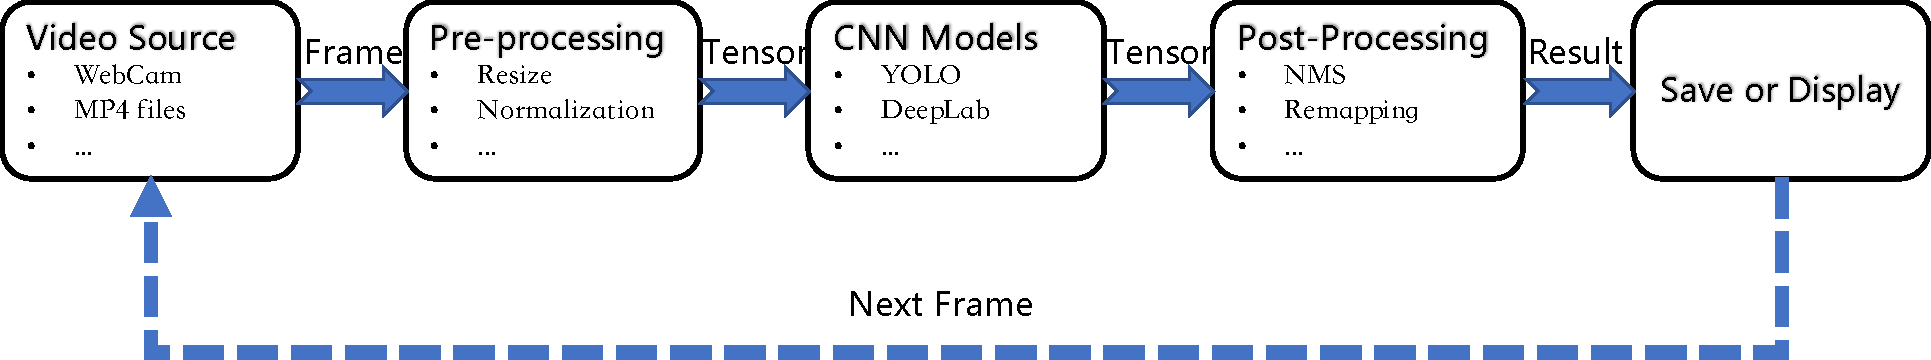
\includegraphics[width=\textwidth]{figure/video_proc_flow.pdf}
    \bicaption{深度学习下视频流处理的一般流程}{Genral process of deep learning based video processing workflow}
    \label{fig:video_proc_flow}
\end{figure}
在深度学习技术的背景下,这些视频分析任务虽然会使用到不同的机器学习算法的组合,但是也存在着许多共通的处理流程。% (emmm,可以考虑加一个流程示意图)
一般情况下,视频流的处理可以看作是在连续的视频帧上做单张图像的视觉计算。因此,视频处理通常由视频流的读取,视频帧的预处理,视觉算法模型(CNN)的运行,算法推理结果的后处理,以及结果的输出与展示这几部分共同来构成,如图\ref{fig:video_proc_flow}所示。当然,对于具体的现实任务来说每一个处理步骤中可能还存在一系列的子步骤,最终会使得整个处理流程的可视化表示变成一个较为复杂的有向无环图(Directed Acyclic Graph,DAG)\footnote{这里不考虑如图\ref{fig:video_proc_flow}中前后帧之间的连接。}。 本文接下来要讨论的视频流处理的优化工作也是基于对视频处理的这种理解与抽象。\par

\section{视频流处理的优化策略}\label{intro_opt}
在\ref{intro_vp}中讨论的视频流处理过程可以进行多层面的优化。从底层硬件到系统运行框架再到算法层面,都有着相应的优化工作。一些相关优化工作也会在第\ref{related_work}章做进一步的讨论。因此本部分仅对相关优化策略做简单介绍:\par

\subsection{针对整体处理流程的系统优化。}\label{sub:sys_opt}
对于像图\ref{fig:video_proc_flow}所示的视频处理过程,由于其存在多阶、相互依赖的连续数据处理的特点,视频处理算法的部署可以参考现代CPU流水线式的处理逻辑,通过多级流水线的模式来部分掩藏处理流程中瓶颈模块的计算耗时。另一方面,对于较复杂DAG连接的视频处理任务,其任务本身就存在一定的并行度,可同时对多个模块并行处理。
\subsection{针对视频特性的视觉算法优化}\label{sub:algo_opt}
现有的深度学习视频分析处理算法多数是直接对视频中的每一帧单独运行原本应用在图像上的视觉算法模型,较少考虑视频帧与帧之间连贯性的特点做算法上的专门优化,从而减少算法在处理过程中的冗余或者非必要计算。在利用视频信息的连贯性上,可引入视频光流估计方法,将前帧的计算结果更快速地传递给后一帧,如Zhu et al.提出的DFF(Deep Feature Flow)模型\cite{zhu2017deep};也可以利用视频编码如H.264\cite{tourapis2003fast}中包含的运动向量(Motion Vector)信息,来对视频关键帧进行选择性检测与传播,如Mao et al.提出的MobiEye\cite{mao2019mobieye};
还可以单纯利用短时间内物体的位移量较小的特点,直接利用上一帧的检测结果,进行接下来的细粒度检测,如Google 的人手追踪模型\cite{mediapipe_hand}。此外,也可利用视频帧的上下文信息来提升视频单帧的检测精度\cite{zhu2017flow}。
\subsection{针对神经网络推理的加速优化}\label{sub:infer_opt}
整个深度学习视频处理流程中的速度瓶颈往往是在神经网络模型的推理步骤上,如\ref{intro_dl}中所说,深度神经网络的推理通常需要进行大量的矩阵计算,有数倍于传统计算处理步骤的时间开销。因此在近年来关于神经网络的压缩,剪枝,量化的研究收到了极大的关注。这些技术从不同的角度对深度神经网络模型精简,在保持模型精度的条件下,尽可能减少模型所需计算资源,提升模型运行速度。此外也有专门针对神经网络推理运算的系统层面的优化加速,比如对需要推理的网络模型进行重编译,对满足特定条件的计算步骤进行融合,从而降低相应算子的调用开销,并优化内存空间的使用。

\subsection{针对模型计算特性的硬件优化}\label{sub:HW_opt}
日渐成熟的深度学习算法的使用也促进了相关硬件平台的发展。深度神经网络所需要进行的矩阵运算对并行计算有着天然的适应性。各大厂商生产的GPU,TPU,VPU等异构芯片在处理这类简单多数据计算时相比传统CPU芯片有着明显的优势。Nvidia在近年来着重发展其GPU产品的AI计算能力,在Volta架构后,为其GPU添加了专门的Tensor Core计算核心来提高其在大量矩阵运算上的处理性能;Google在TPU\cite{jouppi2017datacenter}(Tensor Processing Unit)架构中引入了由大量矩阵乘加器构成的脉动阵列(Systolic Array)结构,来提高矩阵运算的吞吐量;Intel也有推出其集成DSP,VLIW,GPU等特性的混合架构VPU\cite{moloney2014myriad}(Vision Processing Unit),来为移动或边缘设备提供视觉相关AI加速计算的能力。\par~\par

本研究期望对具有一般性的基于深度学习的视频处理任务进行部署与性能上的优化,并通过一种通用框架的形式实现。基于这样的研究目标,我们提出了Accel-Video Pipe (简称AVPipe)这一针对智能视频流处理的编程框架。我们在接下来的框架设计与优化的过程中会主要关注\ref{sub:sys_opt}中介绍的视频流处理在系统层面的优化,同时我们的框架会对现有的神经网络推理优化引擎(\ref{sub:infer_opt})以及相应的计算硬件(\ref{sub:HW_opt})提供充分的支持。对于\ref{sub:algo_opt}中的算法层面优化,由于这类有较强的任务相关性,缺少通用性,故在本框架中不做深入,但用户仍可以通过AVPipe实现相应处理任务的算法优化。

\section{论文的主要内容与章节安排}
本论文大致分为五章展开。在接下来的第二章中,我们将对与本文介绍的视频处理相关的已有优化工作进行介绍,并在其中说明现有相关工作的不足以及可借鉴之处。然后在第三章中,我们将总结现有深度学习相关视频处理任务在实际生产应用中的应用需求以及可能存在的问题,并依此来明确我们的研究动机以及研究目标。
在第四章中,我们将详细介绍我们提出并实现的视频流处理编程框架Accel-Video Pipe,这其中包括AVPipe框架的设计逻辑,主体结构,以及它的自动化部署与优化工具。最后,在第五章中,我们将通过几个示例视频项目的开发,以及性能分析对比,来说明本框架在实际应用过程中的有效性。
\input{tex/floats}
\input{tex/math_and_citations}
% !TEX root = ../thesis.tex

\begin{summary}
本研究课题针对深度学习背景下的视频流处理任务提出了Aceel-Video Pipe(AVPipe)这一C++编程框架,为视频流处理任务提供开发流程与处理速度上的优化。\par
在开发流程上,我们通过对各类视频处理任务进行分析与总结,将整个视频处理任务抽象为数据包(StreamPacket),数据流(Stream),数据处理单元(PipeProcessor)这三者的互联与组合。为此,我们进行了C++相应代码的实现。在实现过程中,我们对处理流程可能涉及的数据类型、数据格式进行了统一与整合;对数据的多线程使用提供了必要的同步与阻塞机制;对多种深度学习推理引擎与计算硬件提供了支持,并简化和统一了调用接口。除了提供较完善的C++库的定义与实现,我们还进一步为便利开发提供了自动化工具。
通过定义处理流程的配置文件,AVpipe可实现自动化的C++代码生成,任务处理流程可视化以及处理流程运行时追踪与分析。\par

在处理速度上,我们为AVPipe提供了针对视频处理任务的多线程优化工具。通过视频处理任务运行时的性能分析,我们可以获得整个处理任务中每一模块的计算用时。多线程优化工具依据这些信息,利用视频处理流程存在的DAG计算模式与流水线计算模式, 将高耗时的瓶颈计算模块划分在不同的线程以实现数据处理的并行化计算。在多线程优化工具的具体实现上,我们提出了有针对视频处理任务特点的启发式DAG处理流程划分算法,在尽可能多线程平摊计算任务的同时,保证多阶段流水线的数据上下依赖关系。\par

最后,通过对一些具体视频处理任务的实现,我们展示了AVPipe的开发流程与性能优化。测试结果表明了我们提出的多线程优化策略的有效性,在某些情境下AVPipe的多线程优化可以提供将近一倍的速度提升。我们之后在GPU与VPU上的测试也进一步展现了AVPipe框架的通用性。\par

AVPipe将会作为一个开源项目在未来继续进行框架的优化与改进。我们会为其持续添加新的计算模块与开发文档;提供可视化的流程连接与参数配置的前端操作界面;移动平台的完善支持;更细粒度的针对视频处理任务的算法与系统层级的优化。我们十分期望AVPipe未来能够在实际生产开发中展现其应有的使用价值。
\end{summary}


% 使用英文字母对附录编号
\appendix

% 附录内容,本科学位论文可以用翻译的文献替代。
\input{tex/app_maxwell_equations}
\input{tex/app_flow_chart}

% 文后无编号部分
\backmatter

% 参考资料
\printbibliography[heading=bibintoc]

% 用于盲审的论文需隐去致谢、发表论文、参与项目、申请专利、简历

% 致谢
% !TEX root = ../thesis.tex

%TC:ignore

\begin{acknowledgements}
\begin{itemize}

\item 感谢冷静文老师对本研究课题的认可与支持!由于毕设的最初研究课题并非“视频流处理优化”,在之后与冷老师沟通,根据个人实际情况在更换为“视频流处理优化”这一课题,没有老师的通融与理解,就不会有如今的毕设论文。其次还要感谢冷静文老师对本项目提供的宝贵指导与意见!这对本毕设的合理开展提供了很大帮助。
  
\item 感谢姚顺宇学长及其创业公司我咖科技团队对本项目的大力支持!选择本课题的很大程度是受学长智能视频应用相关创业项目的影响而选择的。本论文中的测试部分所使用的视频处理任务的CNN模型文件都是由姚学长的团队提供的。我也十分相信的AVPipe框架会在公司今后的视频应用开发上进行实际应用。
  
\item 感谢上海交大学生训练中提供的Nvidia GPU以及Intel Neural Computing Stick 2为本课题带来多样的异构计算资源!
  
\item 感谢所有给予我帮助与鼓励的家人,老师与同学,你们的祝愿是我持续向前的动力!
  
\item 感谢各个图书馆,自习室为我提供的安静且安全的学习环境,尤其是在今年全球疫情这样特殊的情况下,更应值得感激!

\item 感谢 \LaTeX 和 \href{https://github.com/sjtug/SJTUThesis}{\sjtuthesis},为本文排版带来的巨大帮助。

\end{itemize}
\end{acknowledgements}

%TC:endignore


% 发表论文、参与项目、申请专利、简历
% 盲审论文中,发表学术论文及参与科研情况等仅以第几作者注明即可,不要出现作者或他人姓名
\input{tex/publications}
\input{tex/projects}
\input{tex/patents}
\input{tex/resume}

% 中文学士学位论文要求在最后有一个英文大摘要,单独编页码,英文学士学位论文不需要
% !TEX root = ../thesis.tex

\begin{bigabstract}
Artificial Intelligence is absolutely one of the most popular topics in the area of computer science. Recent years have witnessed the fast development of AI-related technologies, especially deep learning technology. Due to its strong feature representation ability, deep learning has gained great success in many important domains such as computer vision, natural language processing and speech recognition, of which computer vision (CV) is the most successful one using deep learning. By using convolutional neural networks (CNNs), deep learning method has achieved great performance in many visual perception challenges including classification, object detection, pose estimation, etc. Thus, deep learning-based computer vision technology is now widely used in production, which can provide convenience to the industry and our daily life. Intelligent video perception is one of the important categories and forms of deep learning-based CV production application. Basically, video perception can be treated as a fixed workflow that continuously processes a specific CV algorithm frame by frame in the video stream. These intelligent video perception tasks are very helpful not only for other advanced AI applications such as autonomous driving and intelligent robotics but also for providing a greater experience for user content creation. 

Though intelligent video stream processing can bring many benefits in real applications, it is relatively difficult to build such video processing pipelines and run it efficiently in users' general computing devices. Firstly, deep learning related video processing tasks usually have complicated processing pipelines containing multiple processing stages related to operations on visual images or high-dimensional tensors. To deploy such pipelines using programming language like C/C++,  you have to write hundreds of or thousands of lines of code, which is pretty hard for those developers without much background knowledge.

Secondly, deep learning, i.e., neural network models usually contain lots of matrix computation which results in more computational resources consumption and more processing time compared to traditional CV methods. Given such characteristics of neural network models, many dedicated software libraries and hardware accelerators are proposed to optimize and accelerate the NN inference process. When we build some video processing pipeline for real-time processing, we may need to select some optimized libraries or hardware for speeding up, which further increases the cost of development.

In order to simplify the development workflow and to optimize the processing speed for intelligent video stream processing tasks, we propose Accel-Video Pipe (AVPipe),  a C++ programming framework aiming to provide better development experience and runtime performance for video stream processing tasks.

Generally, there are 4 strategies to optimize video stream processing tasks, which are: (a) system-level optimization for the overall video processing workflow, e.g. making use of thread parallelism of dependency-free nodes in processing DAG (Directed Acyclic Graph) or multi-stage processing pipeline;  (b) algorithm-level optimization for the overall video processing workflow, e.g. the continuity of visual motion inside consecutive video frames can be used to propagate processing output of one frame to the next frame thus avoid redundant visual computing; (c) processing component level optimization for video processing workflow, especially the optimization for neural network inference component, e.g. model compression, model pruning, model quantization, etc.; (d) hardware-level optimization for video processing workflow, e.g. there are various dedicated neural computing acceleration chips like GPU, TPU, VPU, etc. In order to do some generalized optimizations for a random video stream processing task implemented in AVPipe, we have to choose system-level optimization as our main optimization strategy. Meanwhile, the other strategies are also supported when doing task-related optimization in AVPipe.

To simplify the development workflow, we do a survey on different kinds of video processing tasks to analyze and summarize some common features for the purpose of framework-level data structure abstraction. In our framework, the whole video processing workflow can be treated as a complex combination of 3 basic structures of AVPipe, which are StreamPacket, Stream and PipeProcessor respectively. StreamPacket contains the raw data to be processed; Stream connects different PipeProcessors and directs StreamPacket to its own consumer; PipeProcessor does the actual data processing. To implement these structures in AVPipe, we give special consideration to (a) the integration of different data types and different data formats (e.g. uint8 Mat, float16 Tensor) in StreamPacket structure; (b) necessary thread synchronization and blocking mechanisms to guarantee the data timestamp consistency and avoid race conditions; (c) support for various neural network inference engines and related  computing devices to give simple and unified interface for all libraries of the same function. 

To simplify the development workflow, we do a survey on different kinds of video processing tasks to analyze and summarize some common features for the purpose of framework-level data structure abstraction. In our framework, the whole video processing workflow can be treated as a complex combination of 3 basic structures of AVPipe, which are StreamPacket, Stream and PipeProcessor respectively. StreamPacket contains the raw data to be processed; Stream connects different PipeProcessors and directs StreamPacket to its own consumer; PipeProcessor does the actual data processing. To implement these structures in AVPipe, we give special consideration to (a) the integration of different data types and different data formats (e.g. uint8 Mat, float16 Tensor) in StreamPacket structure; (b) necessary thread synchronization and blocking mechanisms to guarantee the data timestamp consistency and avoid race conditions; (c) support for various neural network inference engines and related computing devices to give a simple and unified interface for all libraries of the same function. 

In addition to the basic definition and implementation of C++ libraries, we provide some automation tools for the further simplification of development. We add an auto code generator to generate the C++ code of a video processing task according to the YAML configuration file formatted by us. Using such configuration files, we can also plot the DAG of the corresponding video processing task. Moreover, a performance profiling tool is implemented to do tracing and timing of different computing component of the whole video processing graph.

To optimize the performance of video processing tasks implemented by our AVPipe, we implement an auto multi-threading optimization tool. There two typical parallelism patterns inside these video processing tasks: parallelism of dependency-free nodes in DAG and parallelism of the multi-stage pipeline with one-sided dependency.  Following these two patterns, our multi-threading optimization tool takes use of tasks' runtime profiling information to filter out some high time-consuming PipeProcessors (i.e., bottleneck processing components) from the video processing graph, and try to make these bottleneck processing components to be placed in separated threads so that some processing time can be overlapped thus processing speed will be improved. When it comes to the actual implementation of our optimization, we propose a heuristic DAG partitioning algorithm to exploit the parallelism patterns mentioned above. In this algorithm, we iteratively put high time-consuming processing components into new threads and do necessary component merging based on the local dependency of these components. There is a theoretic upper bound for our optimization which is the time used by the most time-consuming component, but we may not reach this upper bound for many reasons including the limitation on the number of threads, computation resource contention, complex dependencies among different threads, etc.

We then showcase two video stream processing examples and testify the effectiveness of our multi-threading optimization. The two video processing tasks are pose estimation task and multi-hand tracking task. To show the flexibility of our framework, we also do some CV algorithm level optimization to multi-hand tracking task by adding some user-defined computing components and asynchronous Stream connections. Our test results show that our multi-thread optimization can bring performance improvements for all test cases on different devices including CPU, GPU and VPU. The scale of improvements depends on the complexity of the processing tasks. In some cases, our optimization can even provide almost 1x speedup compared to the corresponding vanilla processing tasks. These promising results prove our AVPipe framework's high effectiveness and high extendability.

As an open-source programming framework, AVPipe will keep adding new functions and improving its supports in the future. We really hope our AVPipe framework will play an important role in the future development of video stream processing applications.

\end{bigabstract}


\end{document}
